\documentclass[12pt,a4paper]{article}

\usepackage[utf8]{inputenc}
\usepackage{ctex}
\usepackage{amsmath,amsfonts,amssymb}
\usepackage{abstract,appendix}
\usepackage{makeidx,hyperref}
\usepackage{graphicx,epsfig,subfig}
\usepackage{geometry}
\usepackage{xcolor}

\geometry{scale=0.8}

%\setlength{\lineskip}{\baselineskip}
\setlength{\parskip}{0.5\baselineskip}

\title{Anderson局部化实验报告5}
\author{flag}
\date{\today}

\begin{document}
    
\maketitle

\section{局部化定位}

这里我们研究K很大,且V为伯努利分布的情况。

研究特征值问题
\begin{eqnarray}\label{e0}
-\Delta u + K V u = \lambda u \qquad \mathbf{x} \in \Omega \\
\frac{\partial u}{\partial n} + h u = 0 \qquad \mathbf{x} \in \partial \Omega
\end{eqnarray}
这个是Robin边界条件,其它边界条件类似。

对于几个最小的特征值和特征函数,在$V(x)=0$的区域内,满足$-\Delta u = \lambda u$,在$V(x)=1$的区域内,满足$-\Delta u + K u = \lambda u$。可以得到
$$ u(x) = \frac{\Delta u(x)}{K-\lambda} $$
由于$K$的数量级远大于$\Delta u(x)$和$\lambda$的数量级,我们可以近似认为,对于前几个较小的特征值,在$V=0$区域内的特征函数为0。

根据之前共振的结论,我们可以把子区域$\Omega_1$选为$V(x)\neq0$的某个连通子区域。考虑子区域上的特征值问题
\begin{eqnarray}
-\Delta u = \lambda u \qquad \mathbf{x} \in \Omega_1 \\
\frac{\partial u}{\partial n} + h u = 0 \qquad \mathbf{x} \in \partial \Omega_1 \cap \partial \Omega \\
u = 0 \qquad \mathbf{x} \in \partial \Omega_1 \setminus \partial \Omega
\end{eqnarray}
如果子区域上的特征值和大区域上的特征值相近,就说明特征函数会localize到这一块子区域。

因此,要判断最小的几个特征值localize到哪片区域,就转化成了\textbf{哪片区域上,拉普拉斯方程的特征值最小?}这样的问题。

对于一维的情况。一维长度为$l$的区间上,Dirichlet边界条件的特征值为$\lambda = \frac{\pi^2}{l^2}, \frac{4 \pi^2}{l^2}, \frac{9 \pi^2}{l^2}, \cdots $。所以想要判断问题localize的区域和特征值大小,只要表示出每个区域上的特征值,然后排序就可以了。

对于原问题为Neumann边界条件的情况,一维长度为$l$的区间上,一半Dirichlet边界一半Neumann边界条件的特征值为$\lambda = \frac{\pi^2}{4 l^2}, \frac{9 \pi^2}{4 l^2}, \frac{25 \pi^2}{4 l^2}, \cdots $。其它部分和Dirichlet边界一样。

因此,主要解决的是二维或者更高维的情况。下面我们分别在Dirichlet边界条件和Neumann边界条件下实验这个问题。下面的图\ref{V}中画出了测试用的势函数$V(x)$,
\begin{figure}[htbp]
\centering
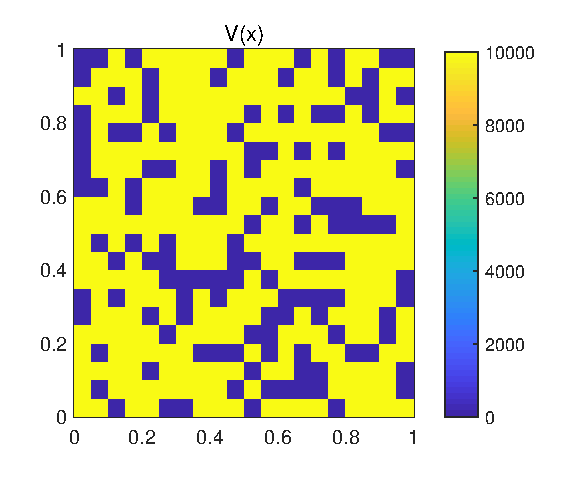
\includegraphics[width=0.4\linewidth]{pics/V}
\caption{势函数}
\label{V}
\end{figure}

\textbf{Dirichlet边界}

首先我们要确保K足够大。我们分别选取$K_1=1.0 \times 10^7$和$K_2=1.1 \times 10^7$模拟问题。表\ref{kD}中列出了在两个参数下特征函数的差别(特征函数归一化到$\max u = 1$)。可以看出,此时继续增大$K$的值,特征函数和特征值变化也不会很大。

\begin{table}
\centering
\begin{tabular}{c|c|c|c}
\hline
特征值序号 & $\max |u_1 - u_2|$ & $|\lambda_1 - \lambda_2|$ & $|\lambda_1 - \lambda_2| / \lambda_2$ \\
\hline
1 & 1.92e-03 & 1.317 & 7.40e-04 \\
2 & 1.82e-03 & 1.309 & 7.33e-04 \\
3 & 3.50e-03 & 3.909 & 1.37e-03 \\
4 & 3.83e-03 & 3.853 & 1.32e-03 \\
5 & 3.45e-03 & 3.982 & 1.34e-03 \\
6 & 3.23e-03 & 3.919 & 1.23e-03 \\
7 & 3.13e-03 & 3.869 & 1.20e-03 \\
8 & 3.21e-03 & 3.831 & 1.17e-03 \\
9 & 3.10e-03 & 3.692 & 1.08e-03 \\
\hline 
\end{tabular}
\caption{验证K足够大}
\label{kD}
\end{table}

我们猜想,Dirichlet边界下,一块区域上最小的特征值和这块区域的(面积/周长)成正比。为了验证这个猜想,我们把区域内所有除了$1\times1$和$1\times2$的子区域都找出来编号,如图\ref{rD}。(这里工作量貌似不大,编号是用人力完成的)

\begin{figure}[htbp]
\centering
\includegraphics[width=0.4\linewidth]{pics/edVD}
\caption{区域编号(Dirichlet边界)}
\label{rD}
\end{figure}

图\ref{eD}中画出了最小的9个特征函数。可以看出,第1,2,3,4,7,9个特征函数,都对应着子区域上的最小特征函数。第5,6个对应区域上第二小的特征函数。第8个对应子区域上第三小的特征函数。

\begin{figure}[htbp]
\centering
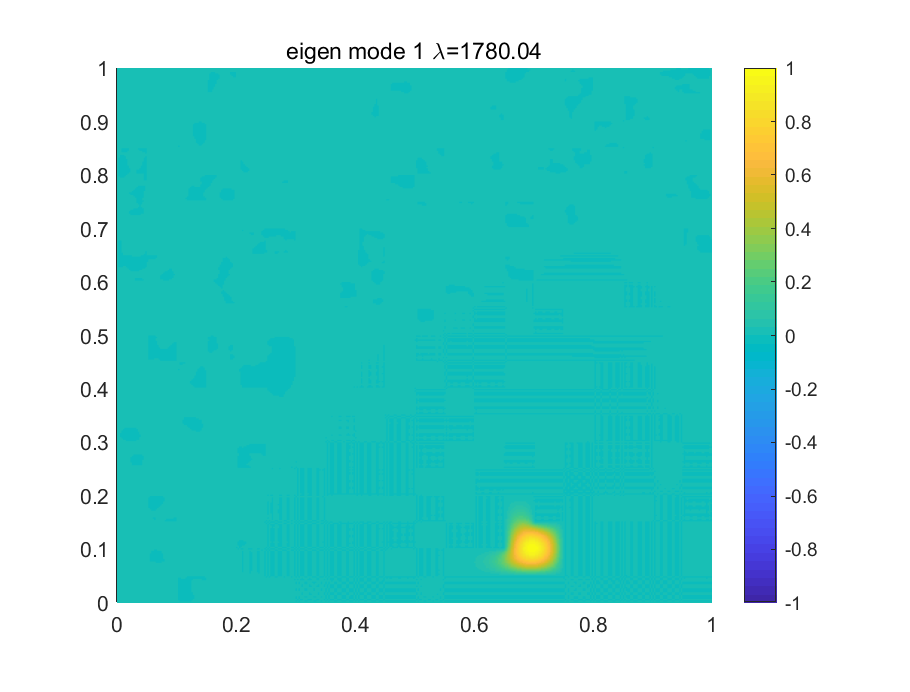
\includegraphics[width=0.3\linewidth]{pics/eigD1}
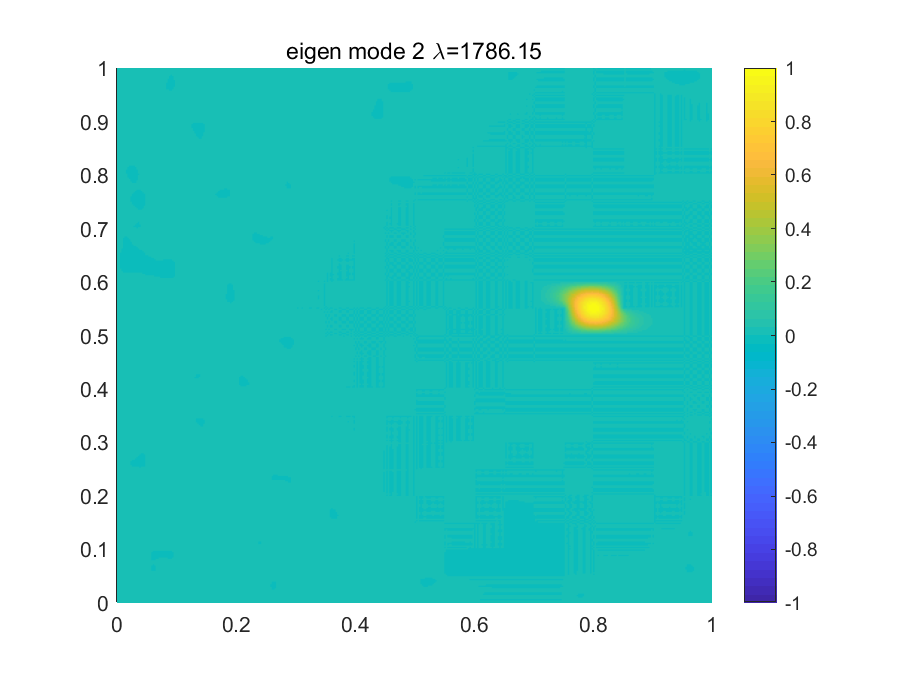
\includegraphics[width=0.3\linewidth]{pics/eigD2}
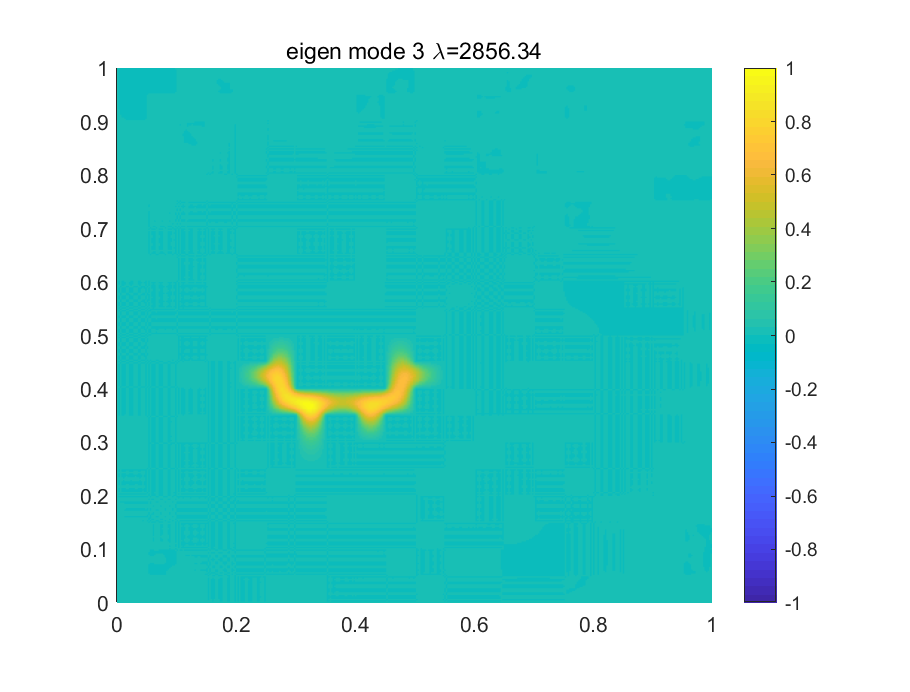
\includegraphics[width=0.3\linewidth]{pics/eigD3}
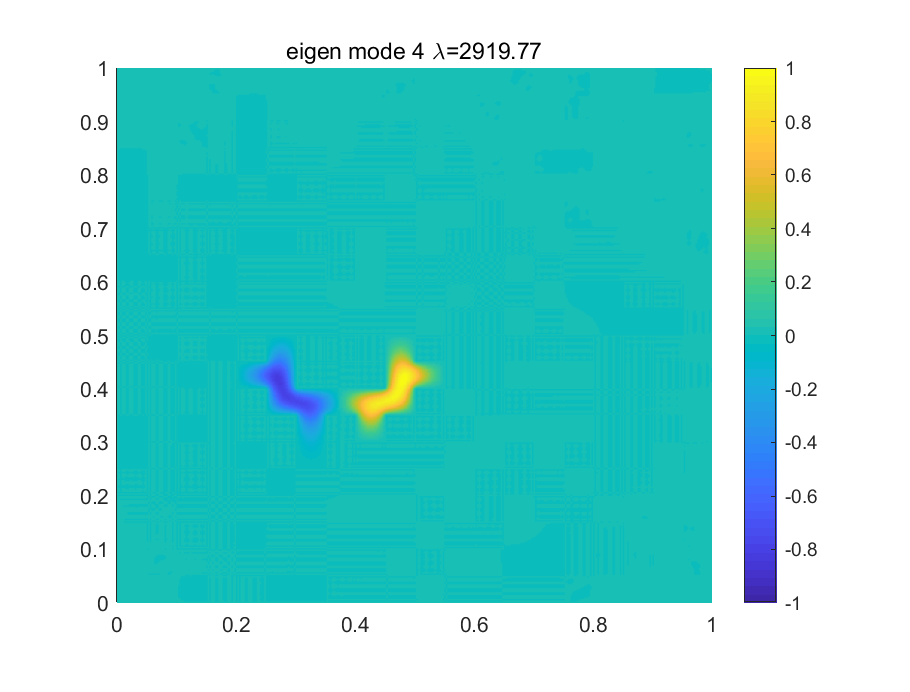
\includegraphics[width=0.3\linewidth]{pics/eigD4}
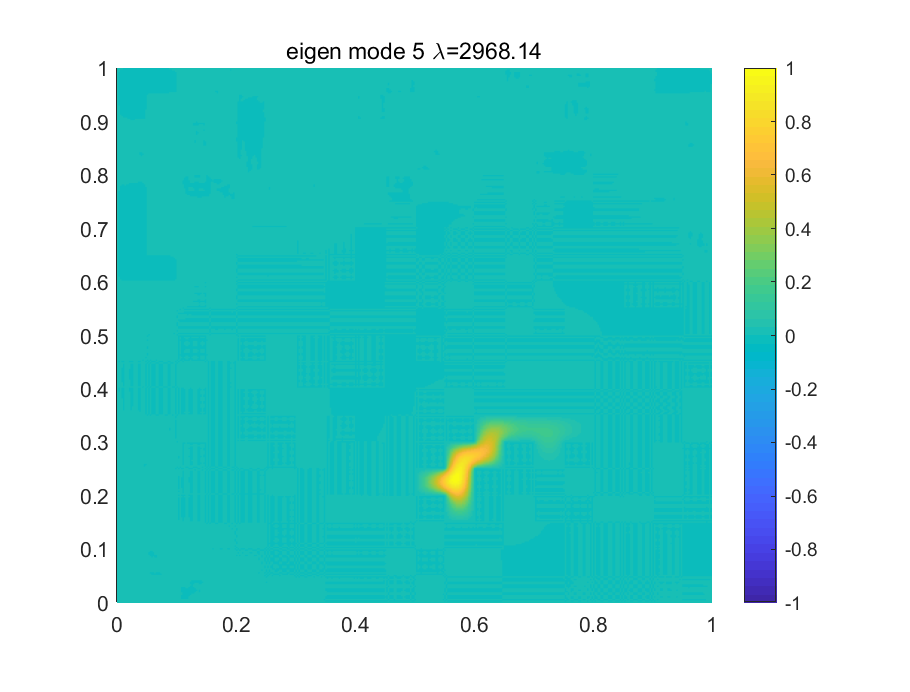
\includegraphics[width=0.3\linewidth]{pics/eigD5}
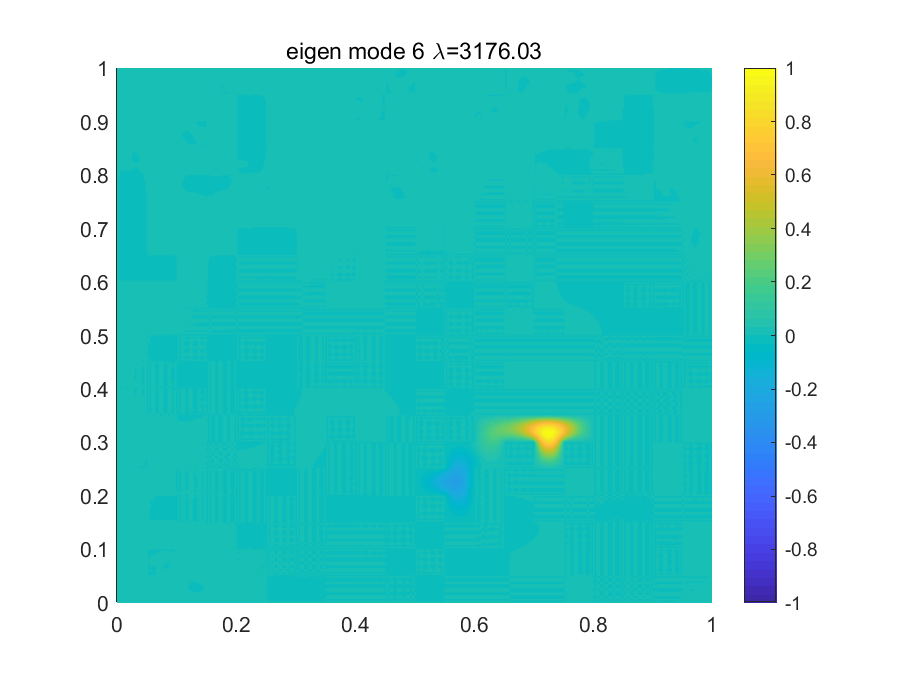
\includegraphics[width=0.3\linewidth]{pics/eigD6}
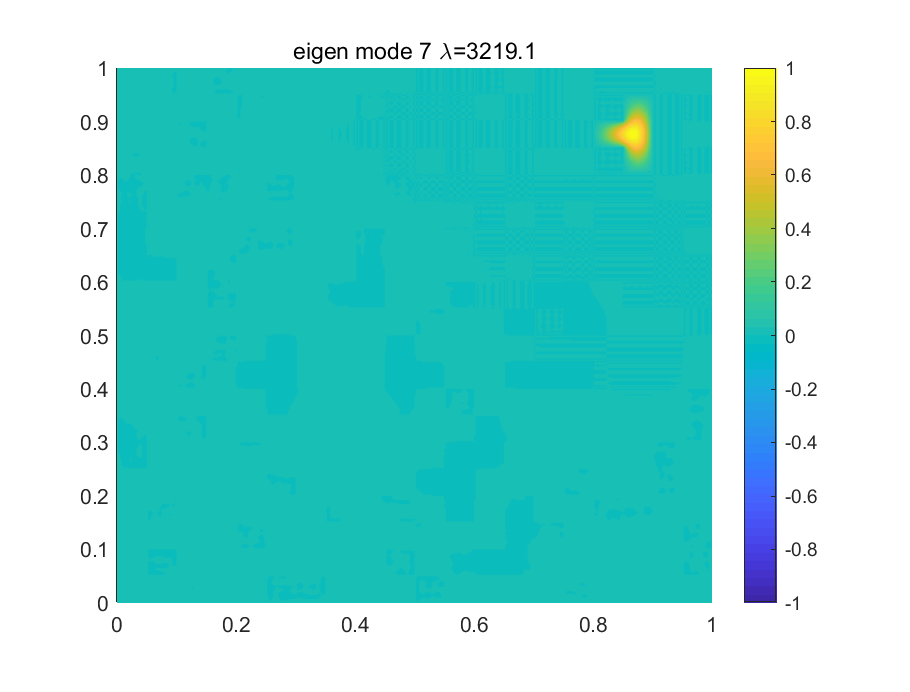
\includegraphics[width=0.3\linewidth]{pics/eigD7}
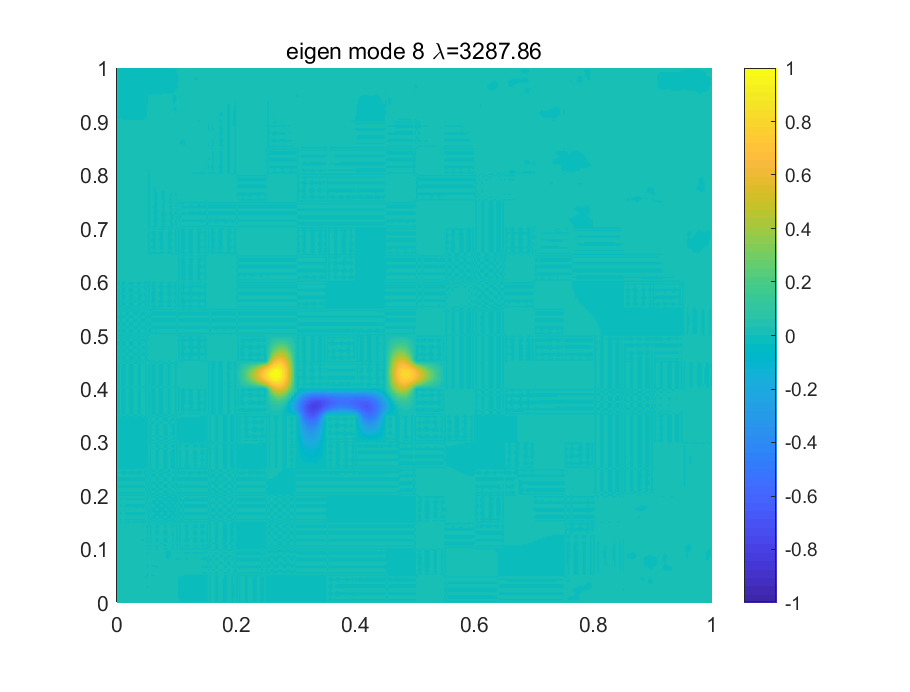
\includegraphics[width=0.3\linewidth]{pics/eigD8}
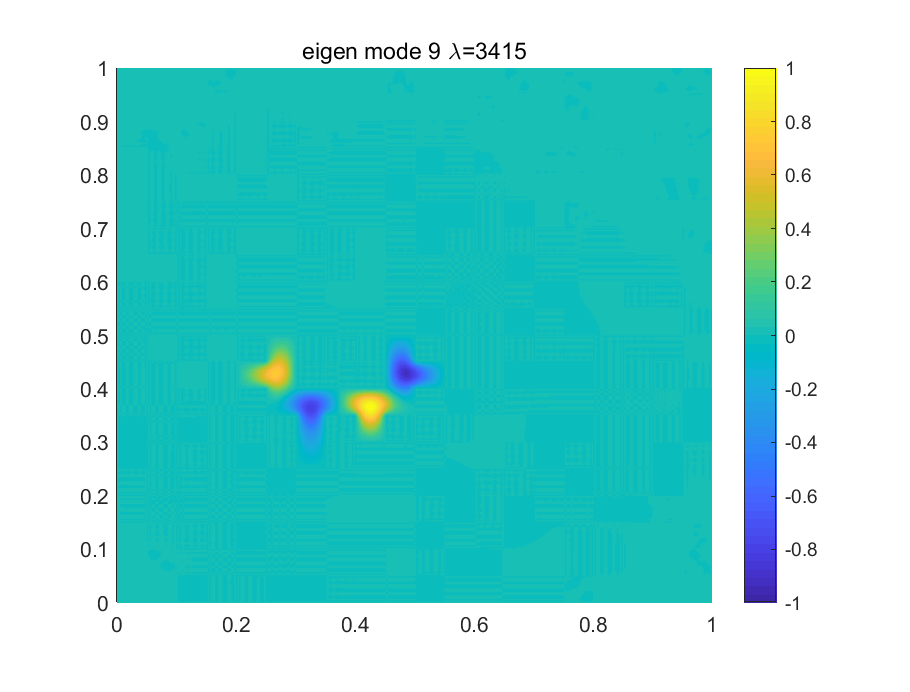
\includegraphics[width=0.3\linewidth]{pics/eigD9}
\caption{Dirichlet边界特征函数}
\label{eD}
\end{figure}

这里需要指出的是:某个区域上,第一个特征值比另一个区域小,其它特征值未必也比另一个区域小。从实验中可以看出,8号区域的第一个特征值比7号和12号都大,但是3号区域上的第二个特征值就比其它区域都小了。所以说,如果有某项近似准则能够判断特征值localize到哪一片区域,也\textbf{只是对特征函数是单峰的情况适用}。

表\ref{tD}中列出了这些区域的周长和面积等信息,可以看出,(面积/周长)确实是一个描述相对趋势的指标,但是这个指标不够精确。4号区域的(面积/周长)很大,但是前9个特征值没有一个聚集在她里面。8号区域看起来形状很奇怪,但是(面积/周长)反而最大。12号区域和10号区域面积和周长完全一样,特征值却相差很大。

\begin{table}
\centering
\begin{tabular}{c|c|c|c|c|c|c}
\hline
编号 & 面积 & 周长 & 面积/周长 & (面积/周长)排名 & 聚集在此处的单峰特征值 & 特征值排名 \\
\hline
8 & 14 & 24 & 0.583 & 1 & 2856 & 3 \\
7 & 7 & 14 & 0.5 & 2 & 1786 & 2 \\
10 & 10 & 20 & 0.5 & 3 & 2968 & 5 \\
12 & 7 & 14 & 0.5 & 4 & 1780 & 1 \\
4 & 6 & 14 & 0.429 & 5 & / & / \\
3 & 4 & 10 & 0.4 & 6 & 3219 & 7 \\
6 & 4 & 10 & 0.4 & 7 & / & / \\
1 & 3 & 8 & 0.375 & 8 & / & / \\
2 & 3 & 8 & 0.375 & 9 & / & / \\
5 & 3 & 8 & 0.375 & 10 & / & / \\
9 & 3 & 8 & 0.375 & 11 & / & / \\
11 & 3 & 8 & 0.375 & 12 & / & / \\
\hline 
\end{tabular}
\caption{Dirichlet边界区域统计}
\label{tD}
\end{table}

综上所述,我们还需要找到一些更有效的指标来刻画它。

\textbf{Neumann边界}

首先我们要确保K足够大。选取同样的参数实验,结果见表\ref{kN}。

\begin{table}
\centering
\begin{tabular}{c|c|c|c}
\hline
特征值序号 & $\max |u_1 - u_2|$ & $|\lambda_1 - \lambda_2|$ & $|\lambda_1 - \lambda_2| / \lambda_2$ \\
\hline
1 & 1.56e-03 & 0.402 & 5.42e-04 \\
2 & 1.07e-03 & 0.678 & 6.05e-04 \\
3 & 4.93e-04 & 0.694 & 5.67e-04 \\
4 & 4.93e-04 & 0.830 & 5.34e-04 \\
5 & 1.92e-03 & 1.317 & 7.40e-04 \\
6 & 1.82e-03 & 1.309 & 7.33e-04 \\
7 & 4.93e-04 & 1.233 & 6.29e-04 \\
8 & 4.93e-04 & 1.233 & 6.29e-04 \\
9 & 4.93e-04 & 1.233 & 6.29e-04 \\
\hline 
\end{tabular}
\caption{验证K足够大}
\label{kN}
\end{table}

对于Neumann边界,我们注意到边界上的对称性。在一维的情况下,一半是Neumann边界一半是Dirichlet边界的区域上,最小的特征值,可以看成把区域进行偶延拓,在两倍长的区域上求解Dirichlet边界的特征值。如图\ref{expand}。因此,我们如果要比较特征值,需要比较子区域沿边界延拓出去之后的新区域上的特征值。\textbf{这个方法就可以解释,为什么对Neumann边界条件,特征函数更容易聚集在边界附近。}

\begin{figure}[htbp]
\centering
\includegraphics[height=0.15\textheight]{pics/DN}
\includegraphics[height=0.15\textheight]{pics/DD}
\caption{混合边界特征函数的延拓}
\label{expand}
\end{figure}

注意,这个延拓只对最小的特征值成立,对第二小的特征值就不成立了。

基于这种猜想,我们把区域内所有除了$1\times1$和$1\times2$在内部的子区域和除了$1\times1$在边界上的子区域都找出来编号,如图\ref{rN}。(这里编号也是用人力完成的)

\begin{figure}[htbp]
\centering
\includegraphics[width=0.4\linewidth]{pics/edVN}
\caption{区域编号(Neumann边界)}
\label{rN}
\end{figure}

同样的势函数$V(x)$下,边界条件为Neumann边界条件。图\ref{eN}中画出了最小的9个特征函数。可以看出,除了第4个特征函数,其它都对应着子区域上的最小特征函数。

\begin{figure}[htbp]
\centering
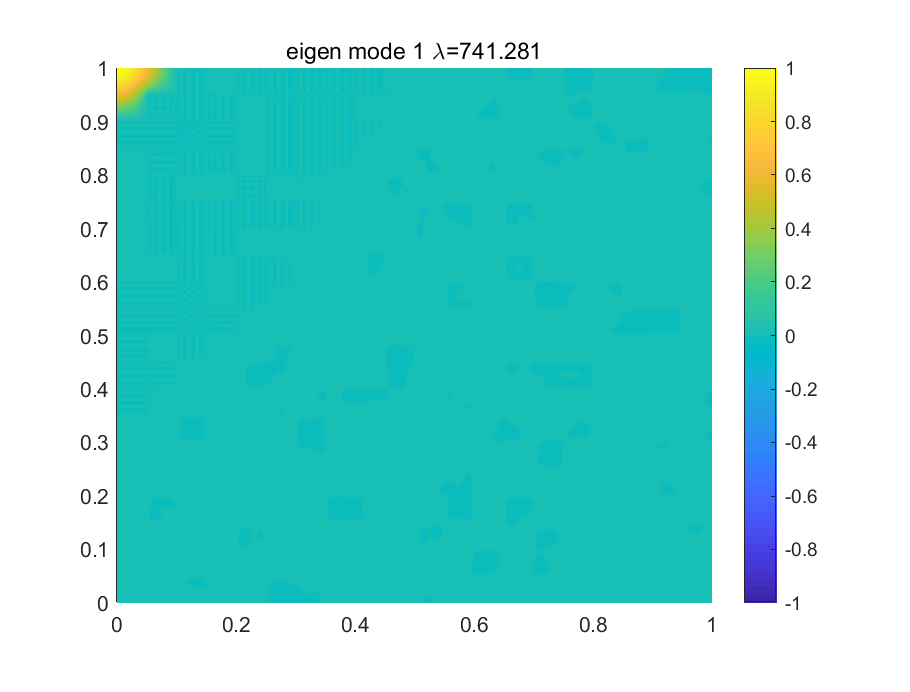
\includegraphics[width=0.3\linewidth]{pics/eigN1}
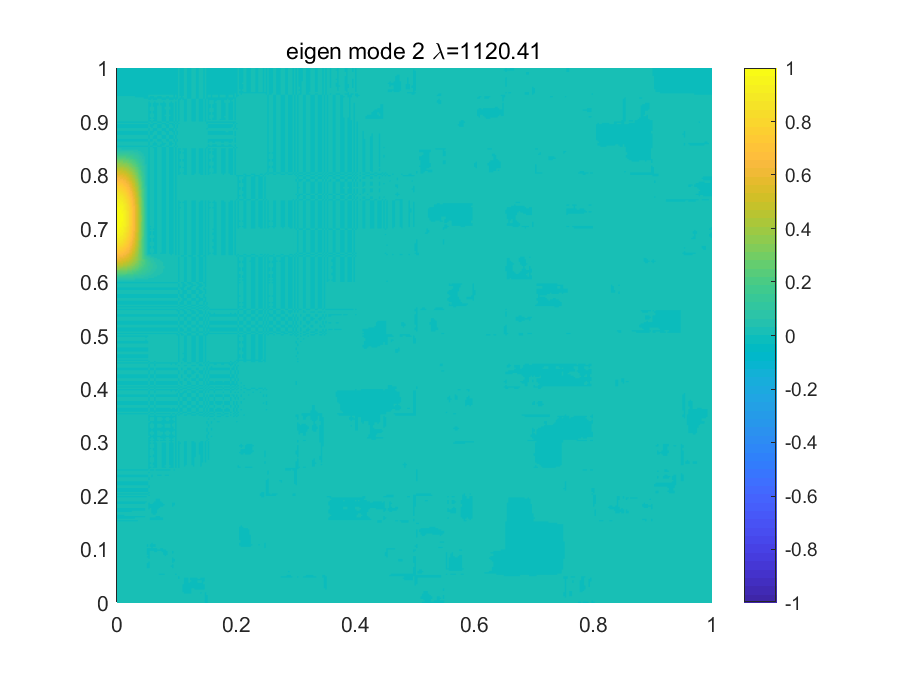
\includegraphics[width=0.3\linewidth]{pics/eigN2}
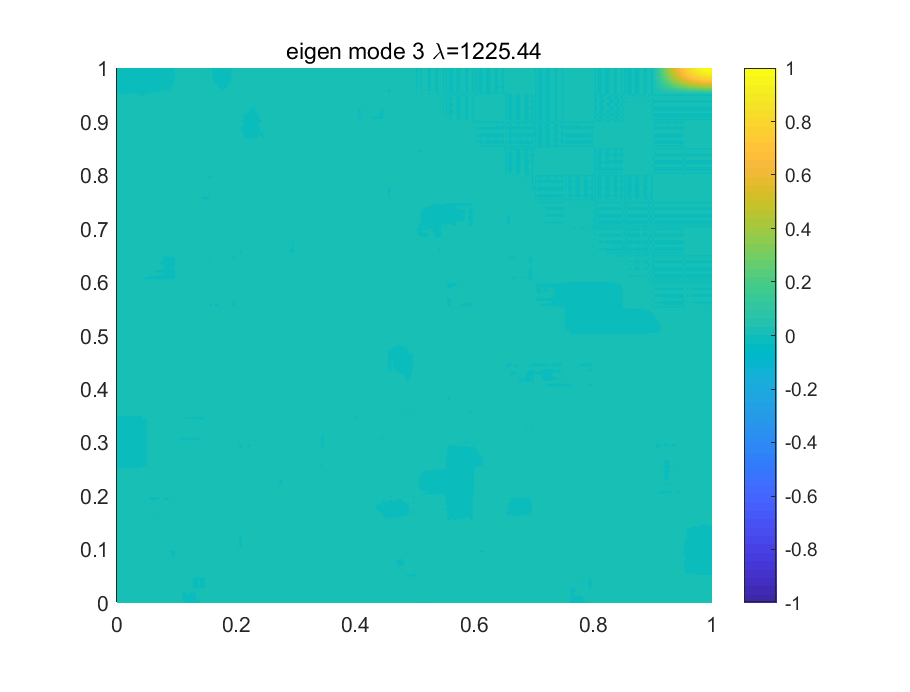
\includegraphics[width=0.3\linewidth]{pics/eigN3}
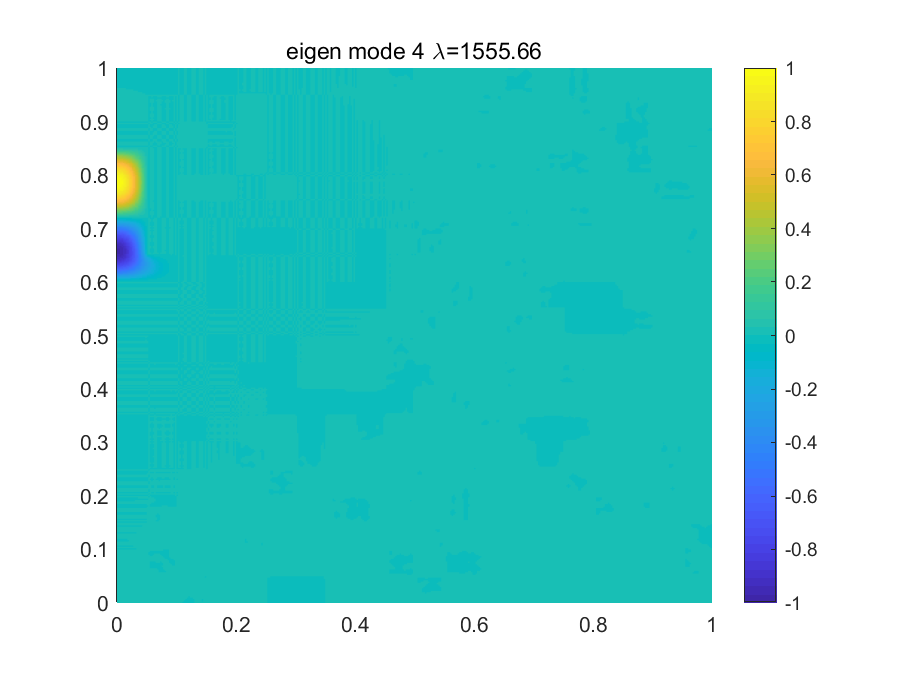
\includegraphics[width=0.3\linewidth]{pics/eigN4}
\includegraphics[width=0.3\linewidth]{pics/eigN5}
\includegraphics[width=0.3\linewidth]{pics/eigN6}
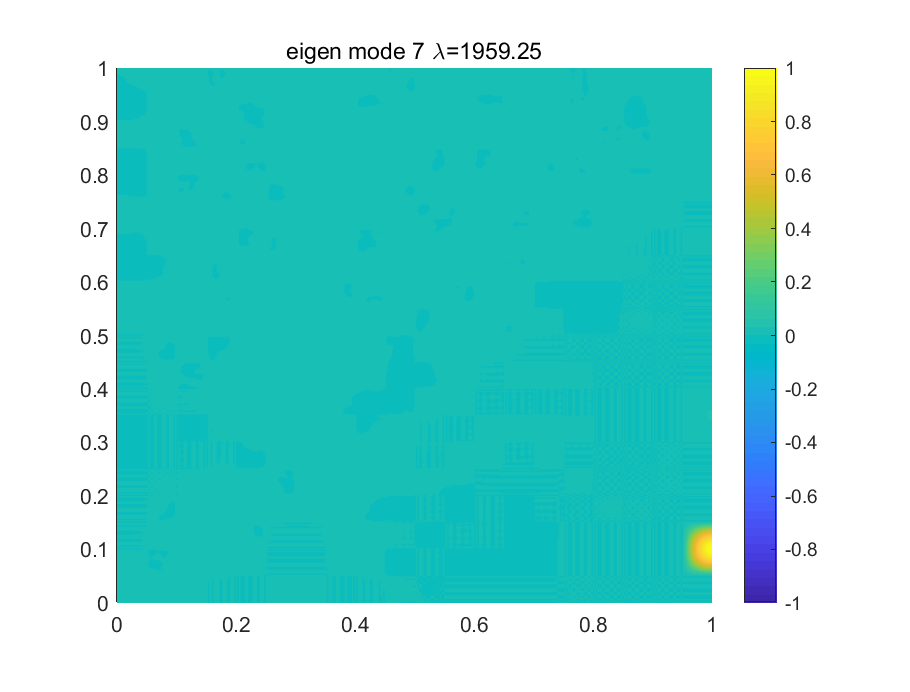
\includegraphics[width=0.3\linewidth]{pics/eigN7}
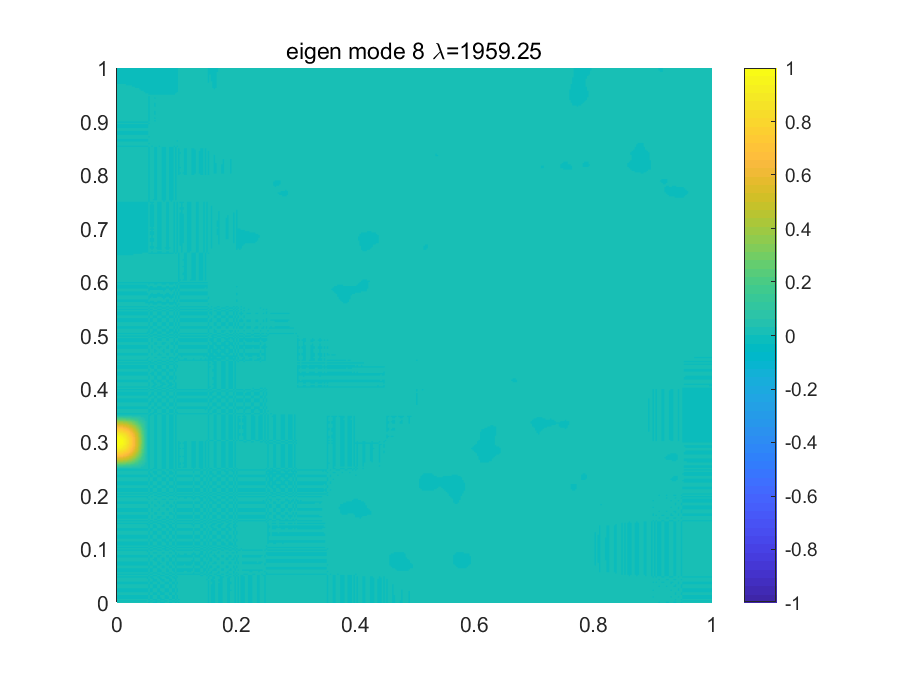
\includegraphics[width=0.3\linewidth]{pics/eigN8}
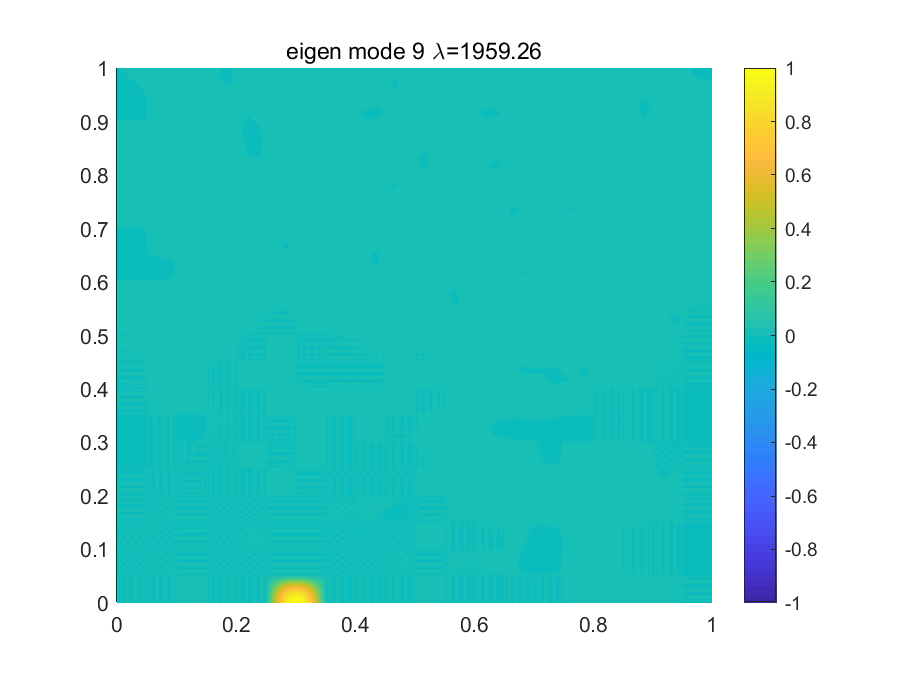
\includegraphics[width=0.3\linewidth]{pics/eigN9}
\caption{Neumann边界特征函数}
\label{eN}
\end{figure}

表\ref{tN}中列出了这些区域的周长和面积等信息。这次效果略好,至少前三个预测对了。第7,8,9,10个特征值也预测对了。

\begin{table}
\centering
\begin{tabular}{c|c|c|c|c|c|c}
\hline
编号 & 面积 & 周长 & 面积/周长 & (面积/周长)排名 & 聚集在此处的单峰特征值 & 特征值排名 \\
\hline
1 & 12 & 16 & 0.75 & 1 & 741 & 1 \\
4 & 12 & 18 & 0.666 & 2 & 1120 & 2 \\
14 & 8 & 12 & 0.666 & 3 & 1225 & 3 \\
8 & 14 & 24 & 0.583 & 4 & / & / \\
7 & 7 & 14 & 0.5 & 5 & 1786 & 6 \\
10 & 10 & 20 & 0.5 & 6 & / & / \\
12 & 7 & 14 & 0.5 & 7 & 1780 & 5 \\
16 & 4 & 8 & 0.5 & 8 & / & / \\
17 & 4 & 8 & 0.5 & 9 & 1959 & 7 \\
18 & 4 & 8 & 0.5 & 10 & 1959 & 9 \\
19 & 4 & 8 & 0.5 & 11 & 1959 & 8 \\
3 & 4 & 10 & 0.4 & 12 & / & / \\
6 & 4 & 10 & 0.4 & 13 & / & / \\
13 & 4 & 10 & 0.4 & 14 & / & / \\
15 & 4 & 10 & 0.4 & 15 & / & / \\
2 & 3 & 8 & 0.375 & 16 & / & / \\
5 & 3 & 8 & 0.375 & 17 & / & / \\
9 & 3 & 8 & 0.375 & 18 & / & / \\
11 & 3 & 8 & 0.375 & 19 & / & / \\
\hline 
\end{tabular}
\caption{Neumann边界区域统计}
\label{tN}
\end{table}

观察到,在不同边界条件下,localize到相同区域的两个特征值是一样的。这可以验证前面的共振理论。

还可以观察到,Neumann边界条件下,16,17,18,19号区域对应的特征值都近似相等,这也可以验证共振的理论。

综上所述,我们还需要找到一些更有效的指标来刻画它。

\textbf{Robin边界:目前还没有办法}

\textbf{结论}
\begin{itemize}
\item K很大时,局部化问题转化成每个子区域上的拉普拉斯特征值问题。
\item 可以用偶延拓的方法把混合Neumann边界的子问题转化为Dirichlet边界的子问题。
\item (面积/周长)这个指标不够准确,我们还要寻找其它指标。
\end{itemize}

\section{effective valley line 的研究}

之前的程序里有错,现在的effective valley line效果很好。仿照PNAS论文里面的图,相同的参数,把边界条件换成Neumann边界条件,得到的结果如图\ref{eVl}。

\begin{figure}[htbp]
\centering
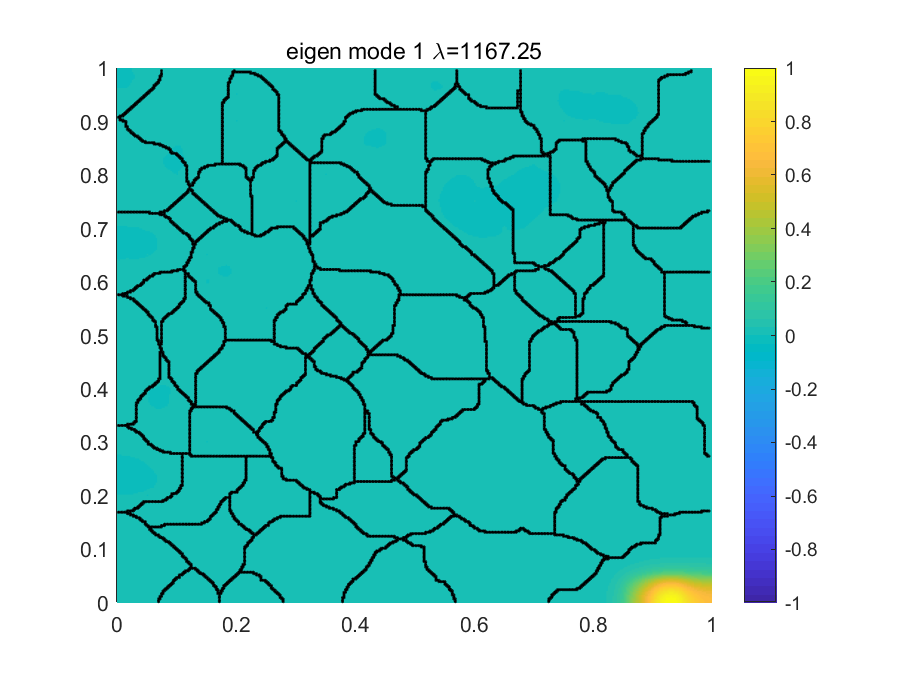
\includegraphics[width=0.3\linewidth]{pics/evl1}
\includegraphics[width=0.3\linewidth]{pics/evl2}
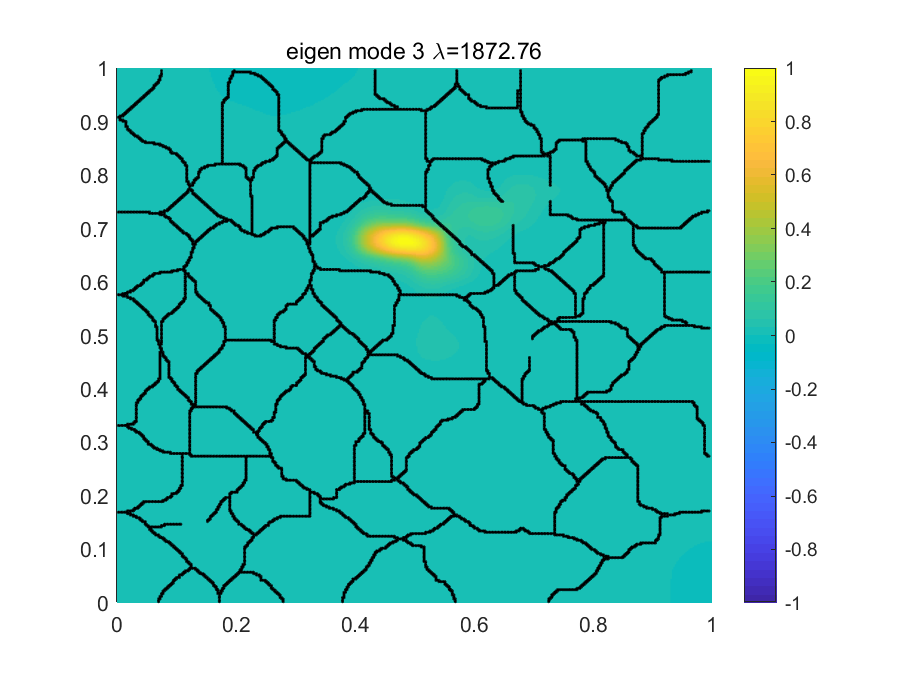
\includegraphics[width=0.3\linewidth]{pics/evl3}
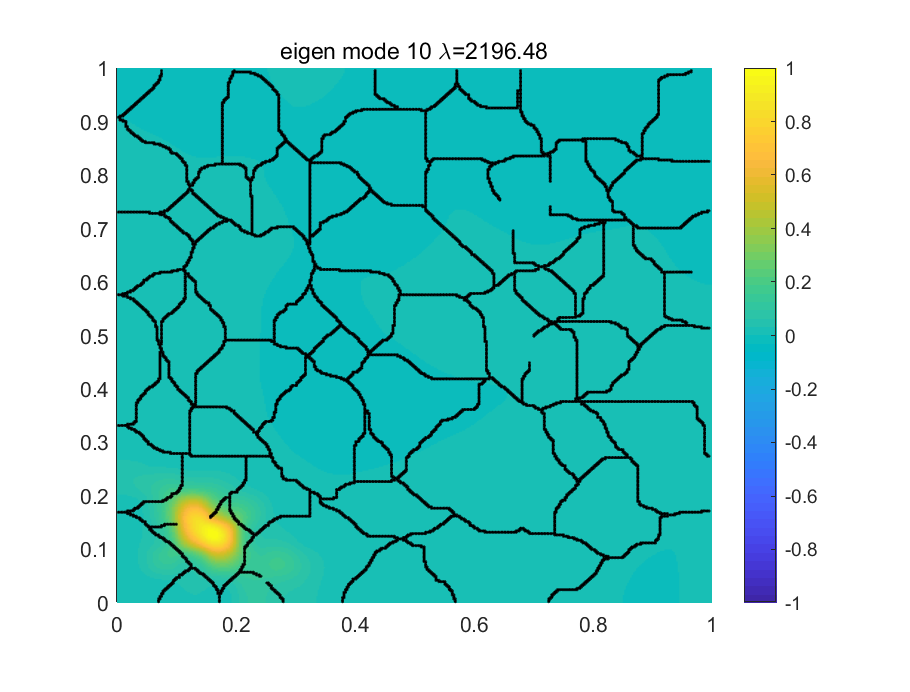
\includegraphics[width=0.3\linewidth]{pics/evl10}
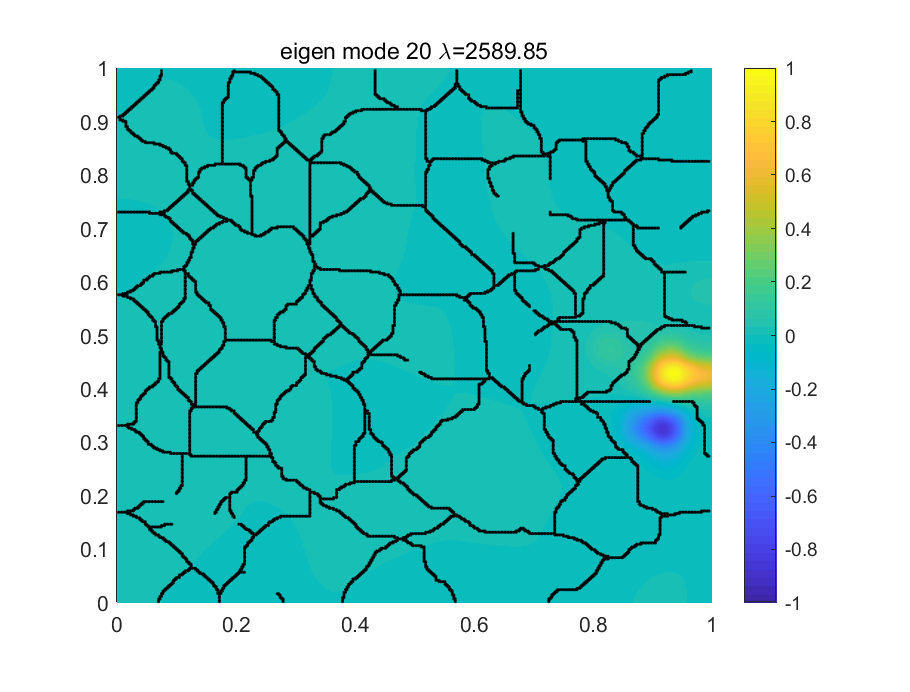
\includegraphics[width=0.3\linewidth]{pics/evl20}
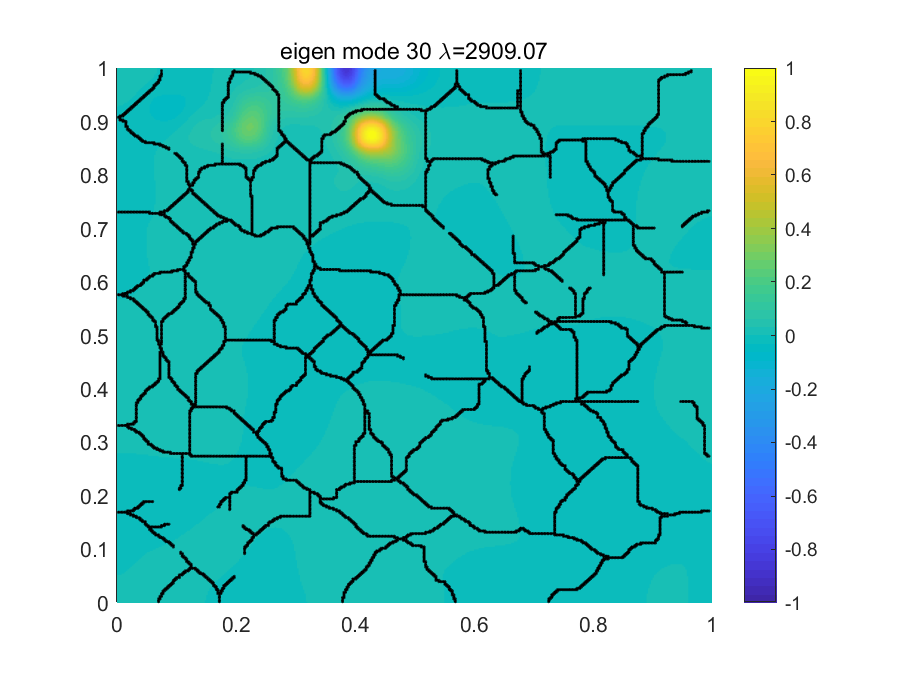
\includegraphics[width=0.3\linewidth]{pics/evl30}
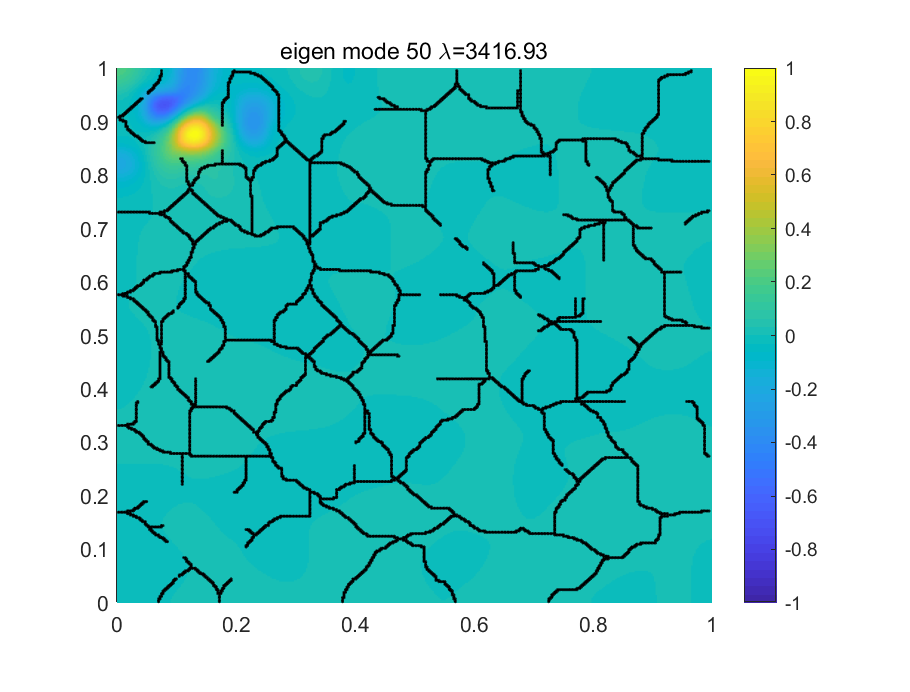
\includegraphics[width=0.3\linewidth]{pics/evl50}
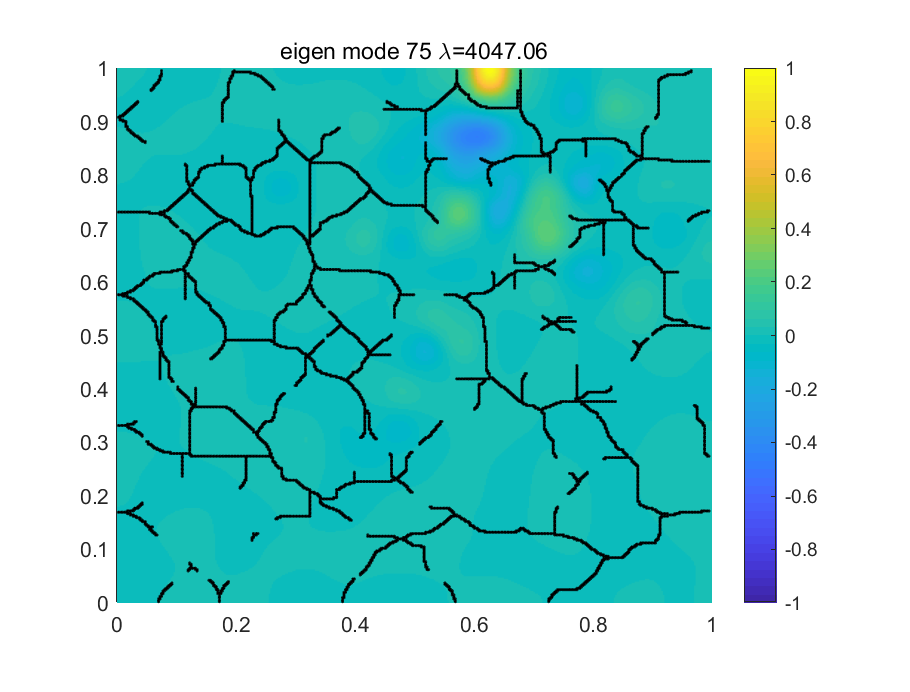
\includegraphics[width=0.3\linewidth]{pics/evl75}
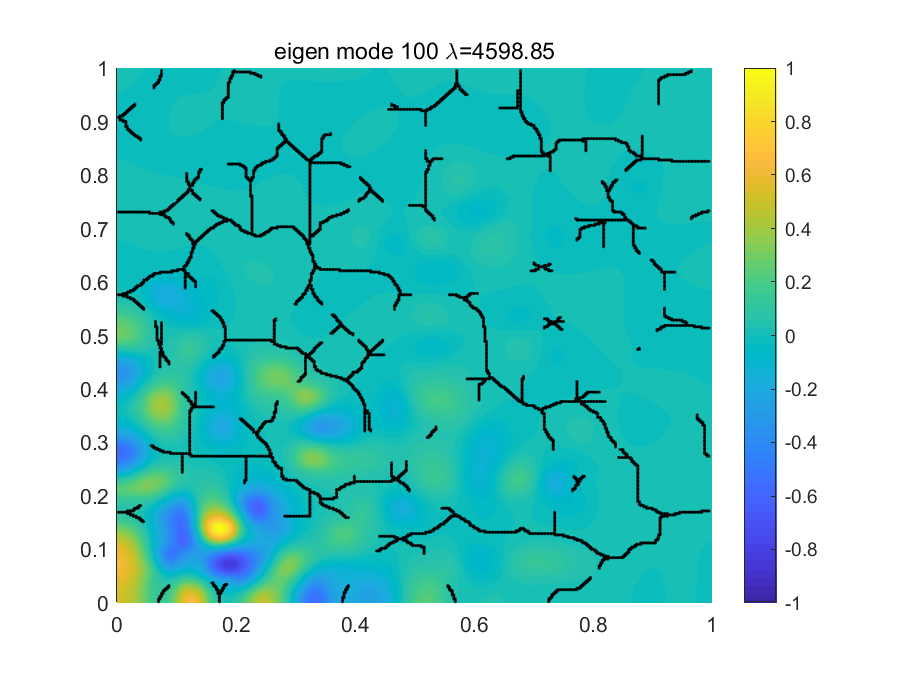
\includegraphics[width=0.3\linewidth]{pics/evl100}
\caption{effective valley line}
\label{eVl}
\end{figure}

\section{谱元法介绍}

我们使用谱元法而不是通常的有限元或者有限差分方法来计算特征函数。谱元法用分片勒让德多项式作为基底逼近方程的精确解,同时限制数值解整体连续。和通常差分方法的误差收敛阶为$\mathcal{O}(h^{-2})$不同,谱元法在这样的问题上可以达到指数收敛,收敛阶为$\mathcal{O}(e^{-N})$。谱元法的计算量只有$\mathcal{O}(M^2 N^2)$,这使得谱元法可以轻易计算大规模的问题。最后,谱元法中的高次多项式可以很好地刻画问题特征函数的奇异性,从而达到更高的精度。本文中我们选择分片10次多项式模拟所有问题。

Eigenmodes are simulated by spectrum elment method instead of ordinary finite element or finite difference method. Legendre polynomials are used in the spectral element method as basis to approximate the solution, while enforce the overall continuty. Ordinary FDM or FEM can only get second-order convergence $\mathcal{O}(h^{-2})$, but the spectral element method can achieve expontial convergence $\mathcal{O}(e^{-N})$ on this problem. Matrix size in spectrual elment method is $\mathcal{O}(M^2 N^2)$, which make it possible for us to simulate large-scale problems. What's more, high degree polynomials can charaterize the singularity of eigenmodes, which can help us attain more accuracy. In this paper, we use picewise polynomial with degree 10 to simulate the following problems.

\end{document}